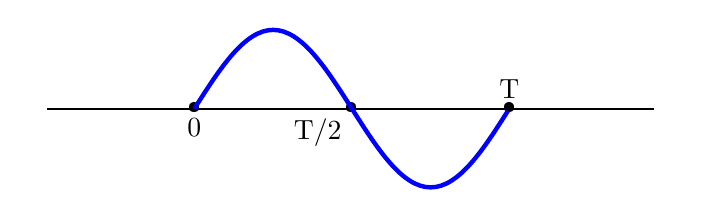
\begin{tikzpicture}[-,shorten >=1pt,auto,node distance=2cm,
  thick,main node/.style={circle,fill=black,draw,font=\sffamily\Large\bfseries}]

\usetikzlibrary{calc}
  
  \node[] (-1) {};
  \node[] (0) [right of=-1] {\textbullet};
  \node[] (1) [right of=0] {\textbullet};
  \node[] (2) [right of=1] {\textbullet};
  \node[] (3) [right of=2] {};
  
  \node[] (0t) [right of=-1, below] {0};
  \node[] (0t) [right of=0, below left] {T/2};
  \node[] (0t) [right of=1, above] {T};


  \path[every node/.style={font=\sffamily\small}]
    (-1) edge node {} (3);
  
  \draw[ultra thick, blue] 
    (0) sin ($(1)+(-1,1)$) cos (1) sin ($(1) + (1,-1)$) cos (2);

\end{tikzpicture}